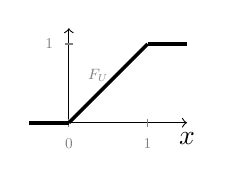
\begin{tikzpicture}
    \draw[->] (-0.5, 0) -- (1.5, 0) node[below] {$x$};
    \draw[->] (0, 0) -- (0, 1.2);
    \foreach \x in {0, 1} {
        \draw [gray] (\x, 0.05) -- ++(0, -.1) ++(0, -.15) node [below, outer sep=0pt, inner sep=0pt, scale=0.6] {\small\(\x\)};}
    \foreach \y in {1} {
        \draw [gray] (0.05, \y) -- ++(-.1, 0) ++(-.15, 0) node [left, outer sep=0pt, inner sep=0pt, scale=0.6] {\small\(\y\)};}
    \draw [gray] (0.5, 0.6) node [left, outer sep=0pt, inner sep=0pt, scale=0.6] {\small\(F_U\)};
    \draw[draw=black,line width=1.3pt] (-0.5,0) -- (0,0);
    \draw[draw=black,line width=1.3pt] (0,0) -- (1,1);
    \draw[draw=black,line width=1.3pt] (1,1) -- (1.5,1);
\end{tikzpicture}